\begin{figure}
    \centering
    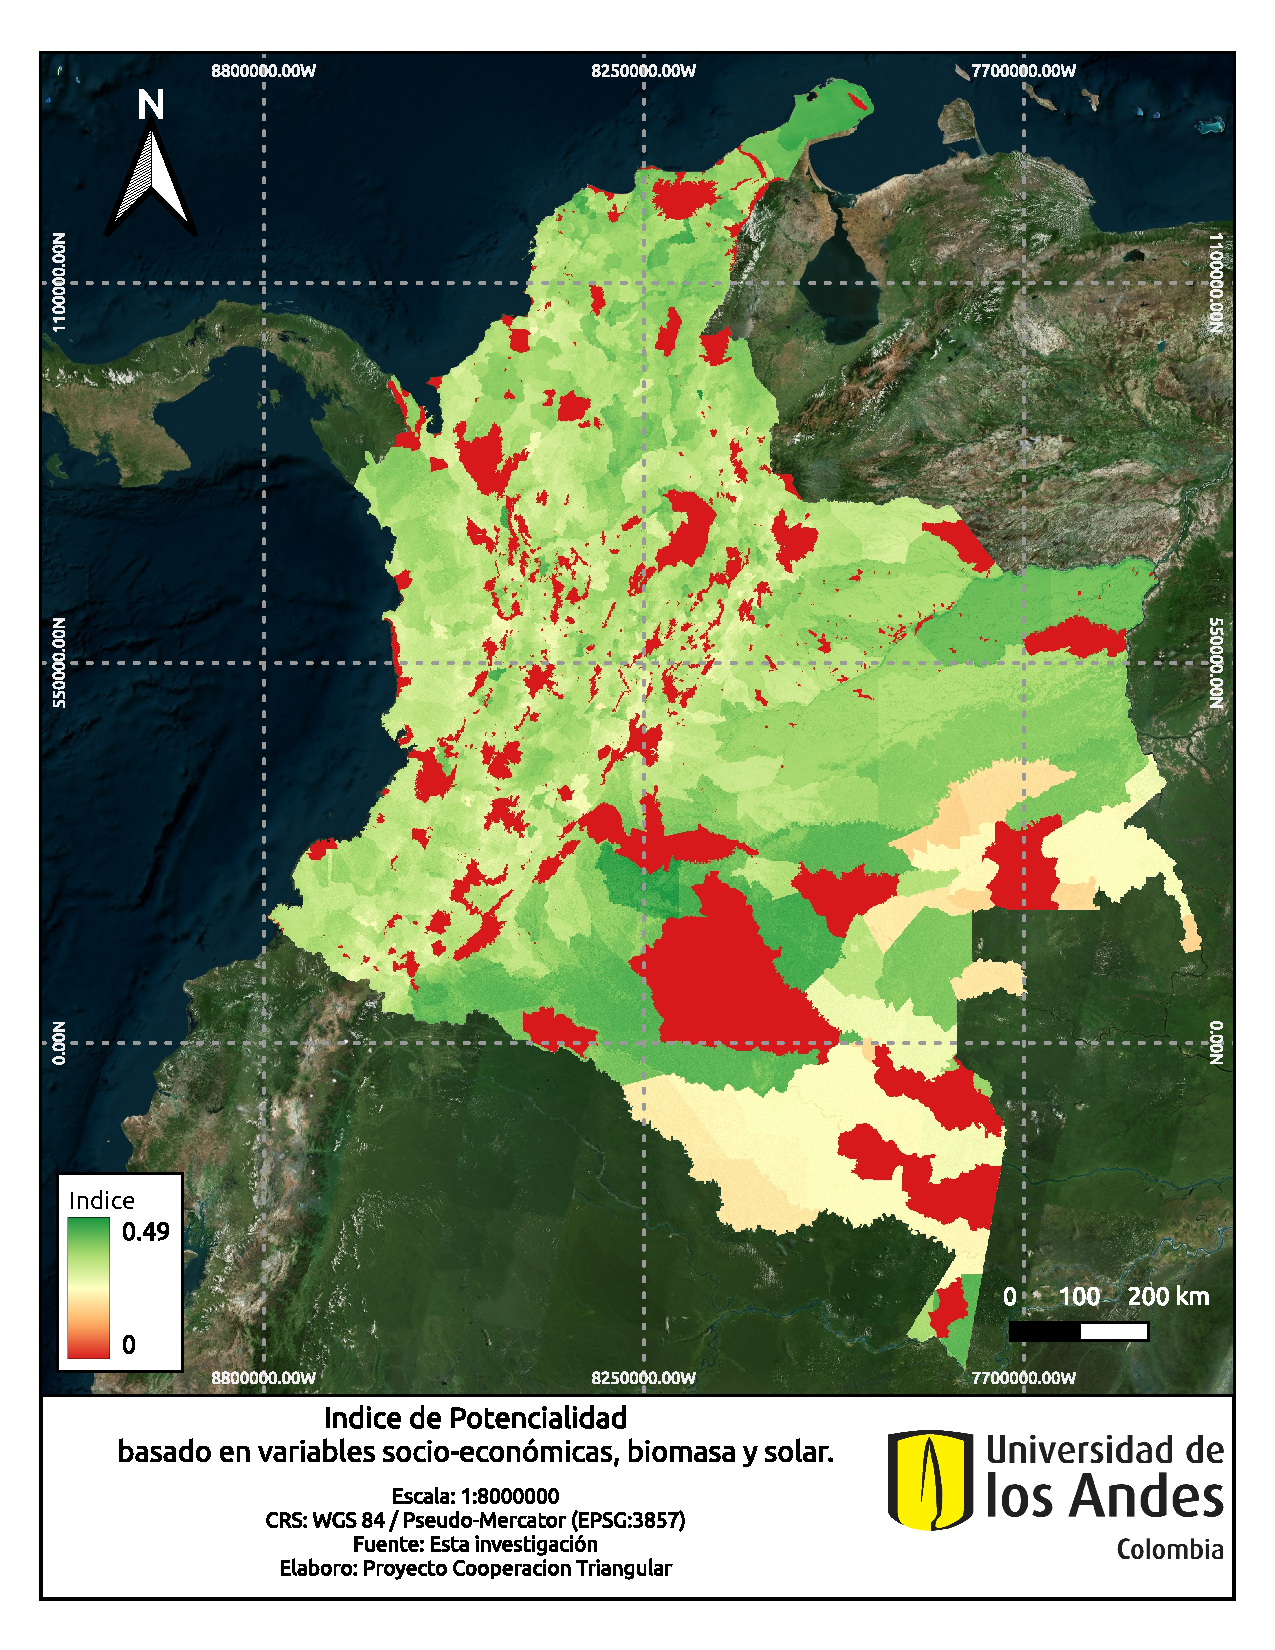
\includegraphics[width=0.95\textwidth]{figures/indice}
    \caption{Indice de potencialidad propuesto.}
    \label{fig:indice}
\end{figure}

\begin{figure}
    \centering
    \includegraphics[width=0.95\textwidth]{figures/pormunicipios}
    \caption{Indice de potencialidad agregado por municipios.}
    \label{fig:pormunicipios}
\end{figure}

\begin{figure}
    \centering
    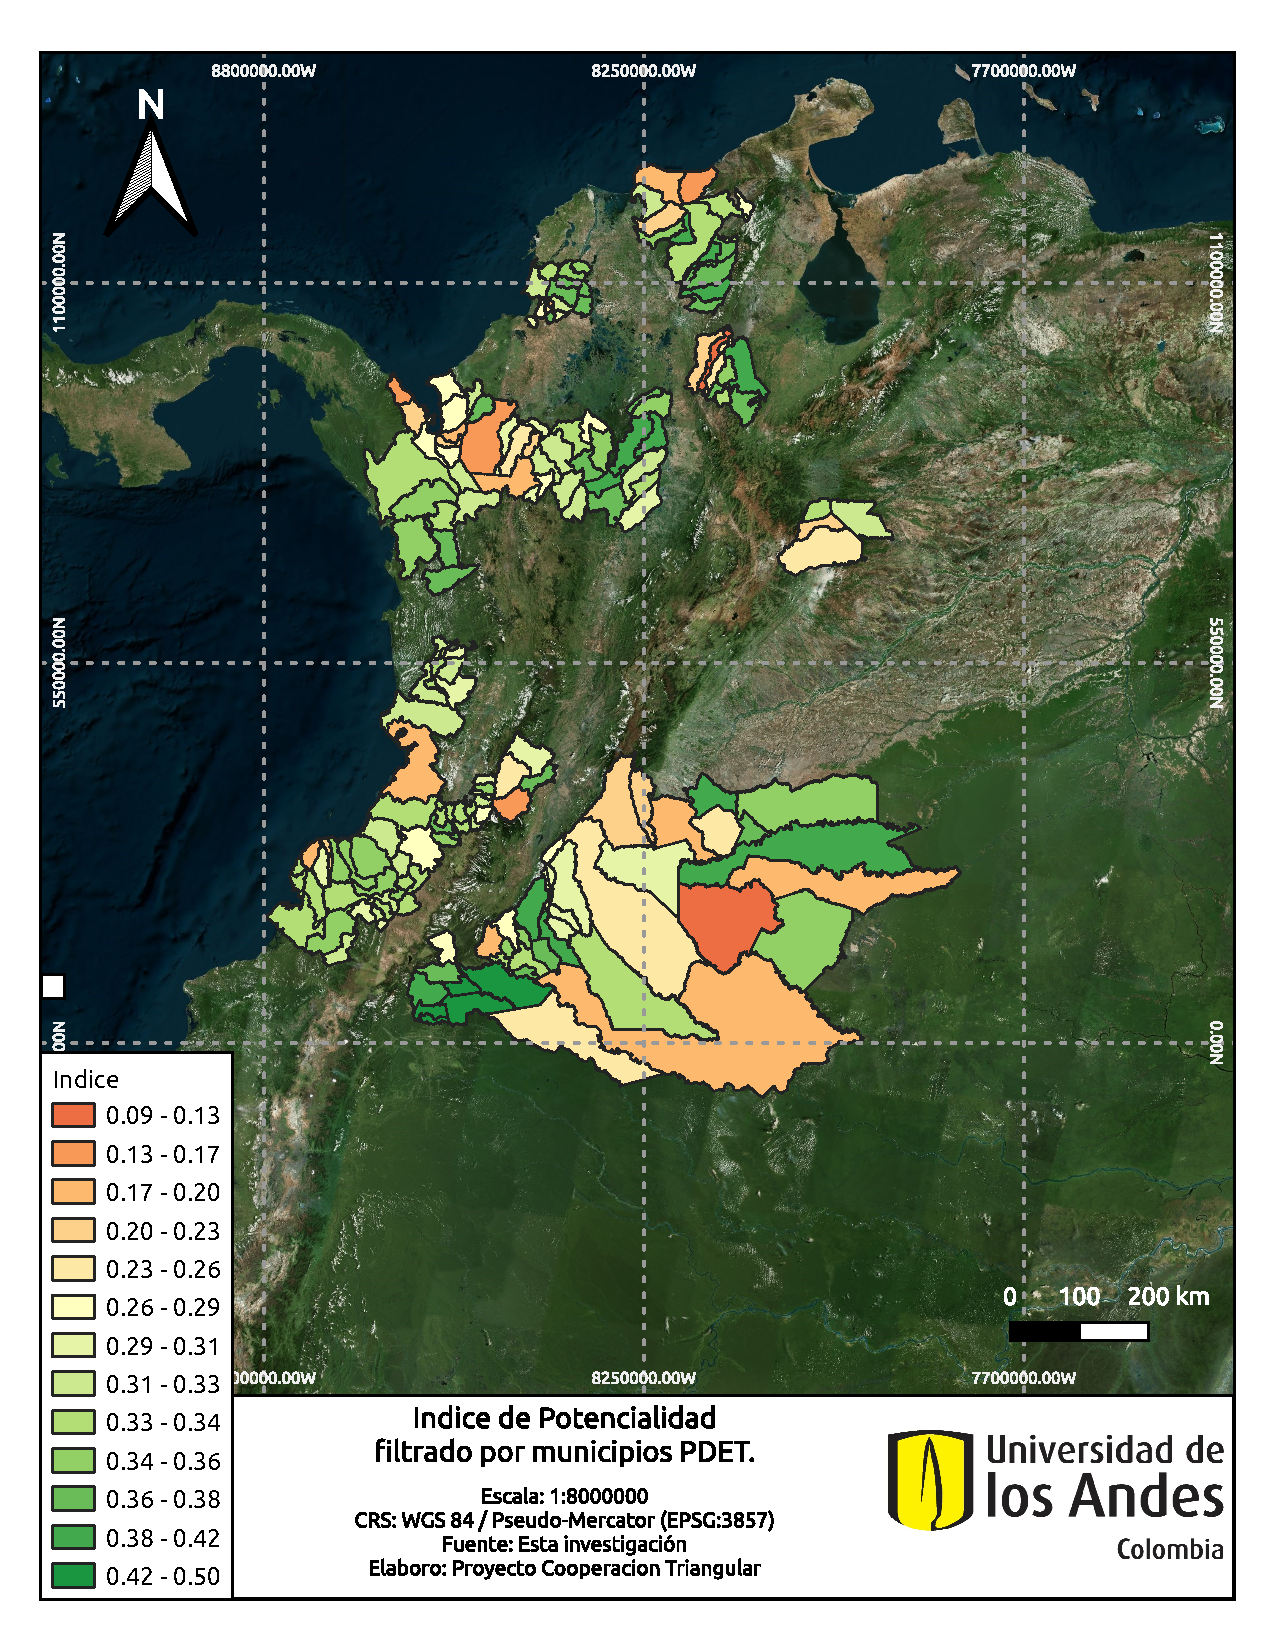
\includegraphics[width=0.95\textwidth]{figures/porpdet}
    \caption{Indice de potencialidad filtrado por municipio PDET.}
    \label{fig:porpdet}
\end{figure}

\begin{figure}
    \centering
    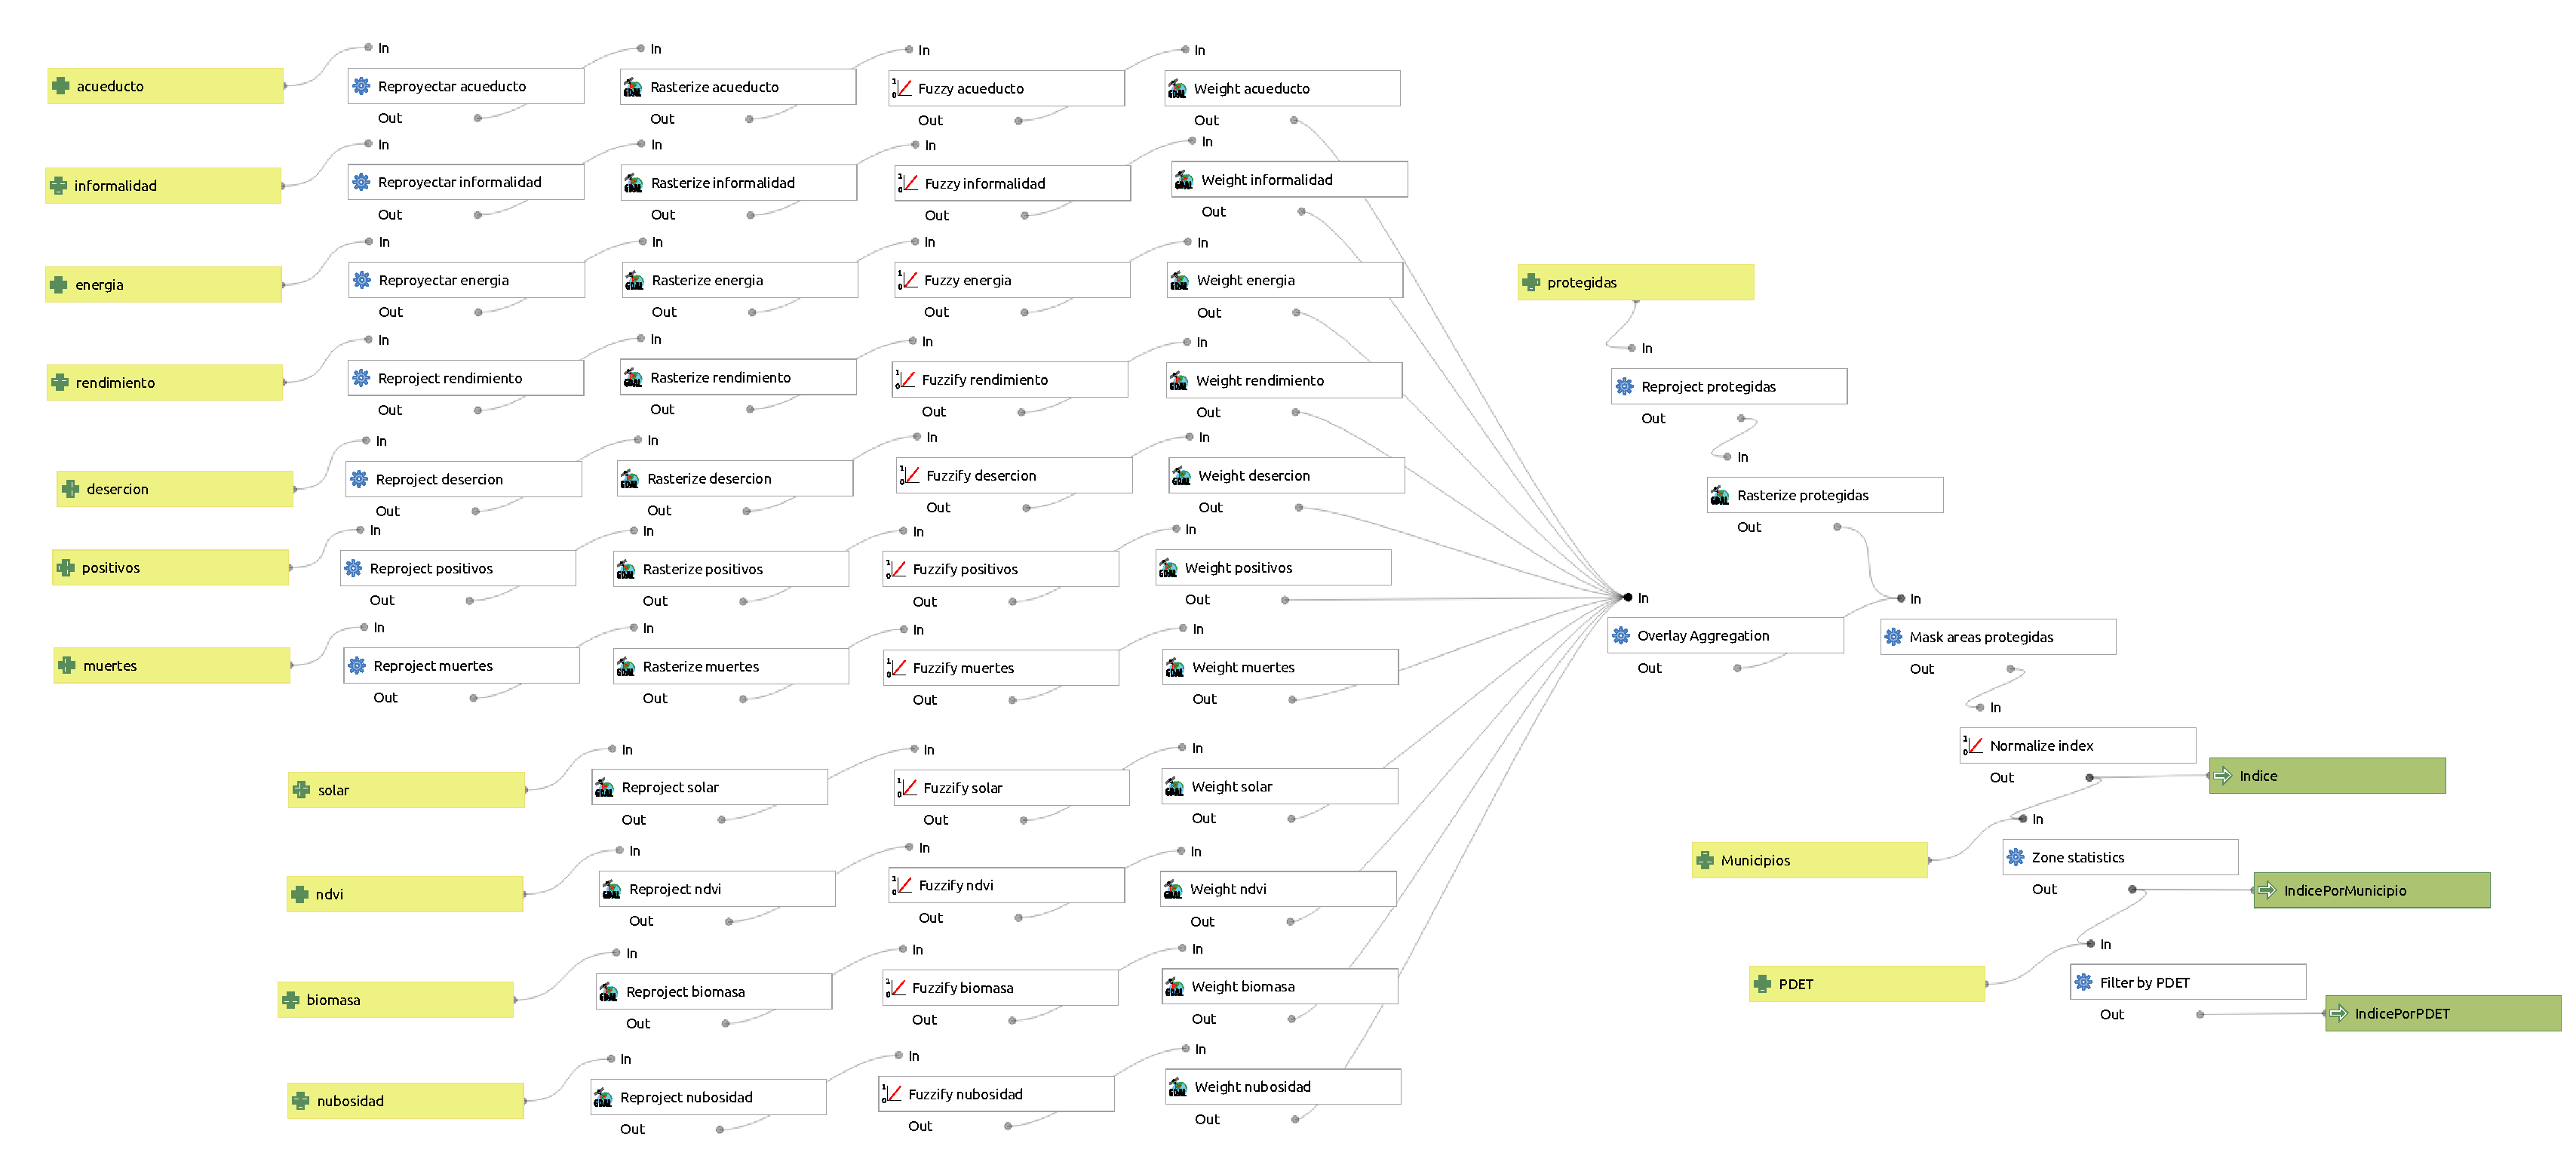
\includegraphics[angle=90, width=0.56\textwidth]{figures/modelo}
    \caption{Modelo QGIS con la implementación de la metodología.}
    \label{fig:modelo}
\end{figure}
